\documentclass{article}

\usepackage[utf8]{inputenc}
\usepackage[T1]{fontenc}
\usepackage[english]{babel}

\usepackage{amsfonts}
\usepackage{amsmath}
\usepackage{amssymb}
\usepackage{authblk}
\usepackage{csquotes}
\usepackage[pdf]{graphviz}
\usepackage{mathtools}
\usepackage{pdfpages}
\usepackage[detect-weight=true]{siunitx}
\usepackage{stmaryrd}
\usepackage{todonotes}

\usepackage[url=false]{biblatex}
\addbibresource{minimum.bib}

\newcommand{\email}[1]{\href{mailto:#1}{#1}}

% Multi-letter identifier
\newcommand{\mli}[1]{\mathit{#1}}

\DeclareMathOperator{\re}{\mathbb{R}}
\DeclareMathOperator{\nat}{\mathbb{N}}
\DeclareMathOperator{\logit}{logit}
\DeclareMathOperator{\sigmoid}{sigmoid}
\DeclareMathOperator*{\argmin}{argmin}
\DeclareMathOperator{\argsort}{argsort}
\newcommand{\inv}[1]{#1^{-1}}
\DeclarePairedDelimiter{\card}{\lvert}{\rvert}
\DeclarePairedDelimiter{\SquareBracket}{[}{]}
\DeclarePairedDelimiter{\Parentheses}{(}{)}
\DeclarePairedDelimiter{\ceil}{\lceil}{\rceil}
\newcommand{\DotProd}[2]{\left<#1,#2\right>}
\newcommand{\Better}[3]{#1 \prec_{#3} #2}
\newcommand{\Prob}[1]{\mathrm{Prob}(#1)}

\DeclareMathOperator{\symbols}{\Sigma}
\newcommand{\Problems}[1]{\mathcal{P}_{#1}}
\DeclareMathOperator{\cnf}{\Problems{\mathrm{CNF}}}
\DeclareMathOperator{\ProblemsTptp}{\Problems{0}}
\DeclareMathOperator{\ProblemsTrain}{\Problems{\mathrm{train}}}
\DeclareMathOperator{\ProblemsTrainEx}{\ProblemsTrain'}
\DeclareMathOperator{\ProblemsVal}{\Problems{\mathrm{val}}}
\DeclareMathOperator{\ProblemsValEx}{\ProblemsVal'}
\newcommand{\signature}[1]{\Sigma_#1}

% Precedences
\newcommand{\PrecBetter}{\pi}
\newcommand{\PrecWorse}{\rho}

\newcommand{\Vampire}{Vampire}

\newcommand{\loss}{\ell}
% Inspiration: The Elements of Statistical Learning, p. 120

\newcommand{\rewrite}[1]{\overset{#1}{\longrightarrow}}

\newcommand{\Conj}{C}
\newcommand{\NegConj}{\mli{NC}}
\newcommand{\AxiomS}{A_s}
\newcommand{\AxiomZ}{A_0}
\newcommand{\RulePS}{R_{+s}}
\newcommand{\RuleSP}{R_{s+}}
\newcommand{\RuleN}[1]{R_{#1}}



\begin{document}

\maketitle

\todo[inline]{Consider qualifying the text as a thesis proposal or a study.}
\todo[inline]{Consider listing the supervisors in the title matter.}

\begin{abstract}
The state-of-the-art superposition-based theorem provers for \acrlong{fol} rely on simplification orderings on terms to constrain the applicability of inference rules,
which in turn shapes the ensuing search space.
The popular Knuth-Bendix simplification ordering is parameterized by symbol precedence---a permutation of the predicate and function symbols of the input problem’s signature.
Thus, the choice of precedence has an indirect yet often substantial impact on the amount of work required to complete a proof search successfully.

This work describes and evaluates two approaches to the construction of a symbol precedence recommender.
Each of them uses machine learning to predict the best possible precedence.
Both recommenders are trained on observations of prover performance on a set of problems and random precedences.
The first approach uses a small set of simple human-engineered symbol features.
The second approach uses a \acrfull{gcn} to extract meaningful symbol embeddings from the graph structure of the input problem.
When coupled with the theorem prover Vampire and evaluated on the \acrshort{tptp} problem library, the \acrshort{gcn}-based recommender is found to outperform a state-of-the-art heuristic by more than \SI{4}{\percent} on unseen problems.

\end{abstract}

\section{Introduction}

Automated theorem proving is a classical field of \gls{ai} \cite{Russell2010}.
Given a sentence written in a formal system such as the \gls{fol},
an \gls{atp} searches for a formal proof of the input sentence.
In the last decades, a number of efficient \glspl{atp} have been implemented,
together with many search heuristics necessary to navigate the search space.
These systems are today increasingly used as black-box reasoners in a number of disciplines.
Such applications include reasoning about all kinds of semantically specified knowledge,
such as mathematics \cite{DBLP:conf/birthday/KinyonVV13},
software and hardware verification \cite{Ahrendt2016}\todo{Cite an example of hardware verification.},
common-sense reasoning \cite{Pease2010},
and legal reasoning \cite{Passmore2017}.

Theorem proving based on the saturation paradigm \cite{DBLP:books/el/RV01/BachmairG01} represents the state-of-the-art method for automatically proving conjectures in \gls{fol}.\todo{Justify the importance of FOL.}
This technology combines several highly nontrivial techniques,
including the use of refutationally complete logical calculi \cite{DBLP:books/el/RV01/NieuwenhuisR01},
powerful redundancy criteria \cite{DBLP:books/el/RV01/BachmairG01},
and advanced indexing \cite{Voronkov1995}.

Despite the ongoing improvements of \gls{atp} systems, with small exceptions,
\glspl{atp} are still significantly weaker than trained mathematicians in finding proofs in most research domains.
At the same time, the area of \gls{ml} and, in particular, the use of deep artificial neural networks has recently seen a number of advances which came hand in hand with several breakthroughs in various application domains.
Examples include \acrlong{cv} \cite{CHAI2021100134},
\acrlong{nlp} \cite{8949185}, and
playing computer games \cite{shao2019survey}.
These recent impressive advances in machine learning manifested in a number of domains suggest to apply such techniques also in the \gls{atp} field.

\section{Related work}

So far, the most successful applications of \gls{ml} in automated theorem proving have been in a high-level external setting of selecting a small number of relevant facts (axioms, definitions, theorems) for proving new conjectures over large formal libraries \cite{DBLP:journals/jar/AlamaHKTU14,DBLP:journals/jar/BlanchetteGKKU16,DBLP:conf/cpp/GauthierK15}.
This has become known as the premise selection task.
More recently, \gls{ml} has also started to be used to guide the internal search of the \gls{atp} systems.
This means providing advice when the \gls{atp} is choosing among many possible inference steps of its non-deterministic proof calculus.
This is more challenging, because the trained machine learner is typically called thousands of times during the proof search and thus needs to be both fast and efficiently integrated with the core \gls{atp} system.
In the simpler connection tableau systems such as leanCoP \cite{10.1007/978-3-540-71070-7_23}, supervised learning has been used to choose the next tableau extension step \cite{DBLP:journals/jar/FarberKU21} and first experiments with Monte-Carlo guided proof search and reinforcement learning have been done, recently outperforming the unguided systems by \SI{40}{\percent} on standard benchmarks \cite{DBLP:conf/nips/KaliszykUMO18}.
In saturation-style provers this has been done by feedback loops for strategy invention \cite{DBLP:journals/aicom/JakubuvU18,DBLP:conf/gcai/SchaferS15} and by using supervised learning \cite{DBLP:conf/cade/JakubuvCOP0U20,DBLP:conf/lpar/LoosISK17} to select the next given clause \cite{McCune2003}.

\todo[inline]{Cite work on simplification orderings (KBO, LPO), precedences (invfreq), GCNs, HPO (?).}

\section{Objectives}
\todo{Consider leaving this section out since it is not required.}

My PhD research is conducted under the joint supervision of
\href{http://people.ciirc.cvut.cz/~sudamar2/}{RNDr. Martin Suda, Ph.D.} and
\href{https://people.ciirc.cvut.cz/~urbanjo3/}{Mgr. Josef Urban, Ph.D.}.\todo{Consider leaving the academic titles out.}

The main objective of my research is an investigation of novel ways of increasing the performance of state-of-the-art saturation-based \glspl{atp} by using \gls{ml}.
The \gls{atp} Vampire \cite{DBLP:conf/cav/KovacsV13} serves as the primary target system of interest
namely due to its relative strength
as testified by the annual \gls{casc} \cite{Sut16}.

While the main goal of the project is improved performance of \gls{atp} systems, the topic is very interesting also from the perspective of general \gls{ai} research. Successful combinations of statistical and symbolic \gls{ai} are still relatively rare, and it is well known that first-order theorem proving is undecidable. This leads to a number of questions about both the theoretical and practical power of existing learning approaches in reasoning tasks. Exploring these limits is the implicit secondary objective of this project.

\section{Results}

The state-of-the-art \gls{fol} \gls{atp} Vampire uses superposition calculus as its inference system.
The superposition calculus is restricted by a simplification ordering on terms,
which is usually parameterized by a symbol precedence -- a permutation of the input problem signature.

The results of this research published so far
comprise the design and evaluation of two methods of recommending symbol precedences:

\begin{enumerate}
\item Learning Precedences from Simple Symbol Features \cite{DBLP:conf/cade/Bartek020}:
A precedence recommender based on simple syntactic symbol features published at \gls{paar-2020}
\item Neural Precedence Recommender \cite{Bartek2021}:
A precedence recommender based on a \gls{gcn} published at \gls{cade-28}
\end{enumerate}

Verbatim copies of these two publications form the last part of this document.

\todo[inline]{Consider adding section Future work. While it is not required by the specification, it may be interesting for the readers, and Zar included such section in his thesis proposal.}

%\section{Future work}

%A typical \gls{atp} such as Vampire uses a large number of parameterized heuristics.
%Given an \gls{atp}, a strategy is a configuration of the prover's parameters.
%Given an input problem, the performance of the prover may vary greatly depending on the chosen strategy.
%The resulting space of admissible strategies is typically too large to enumerate in practice.

%The following part of this research project will focus on the problem of strategy synthesis and schedule synthesis.

\bibliographystyle{plain}
\bibliography{minimum}

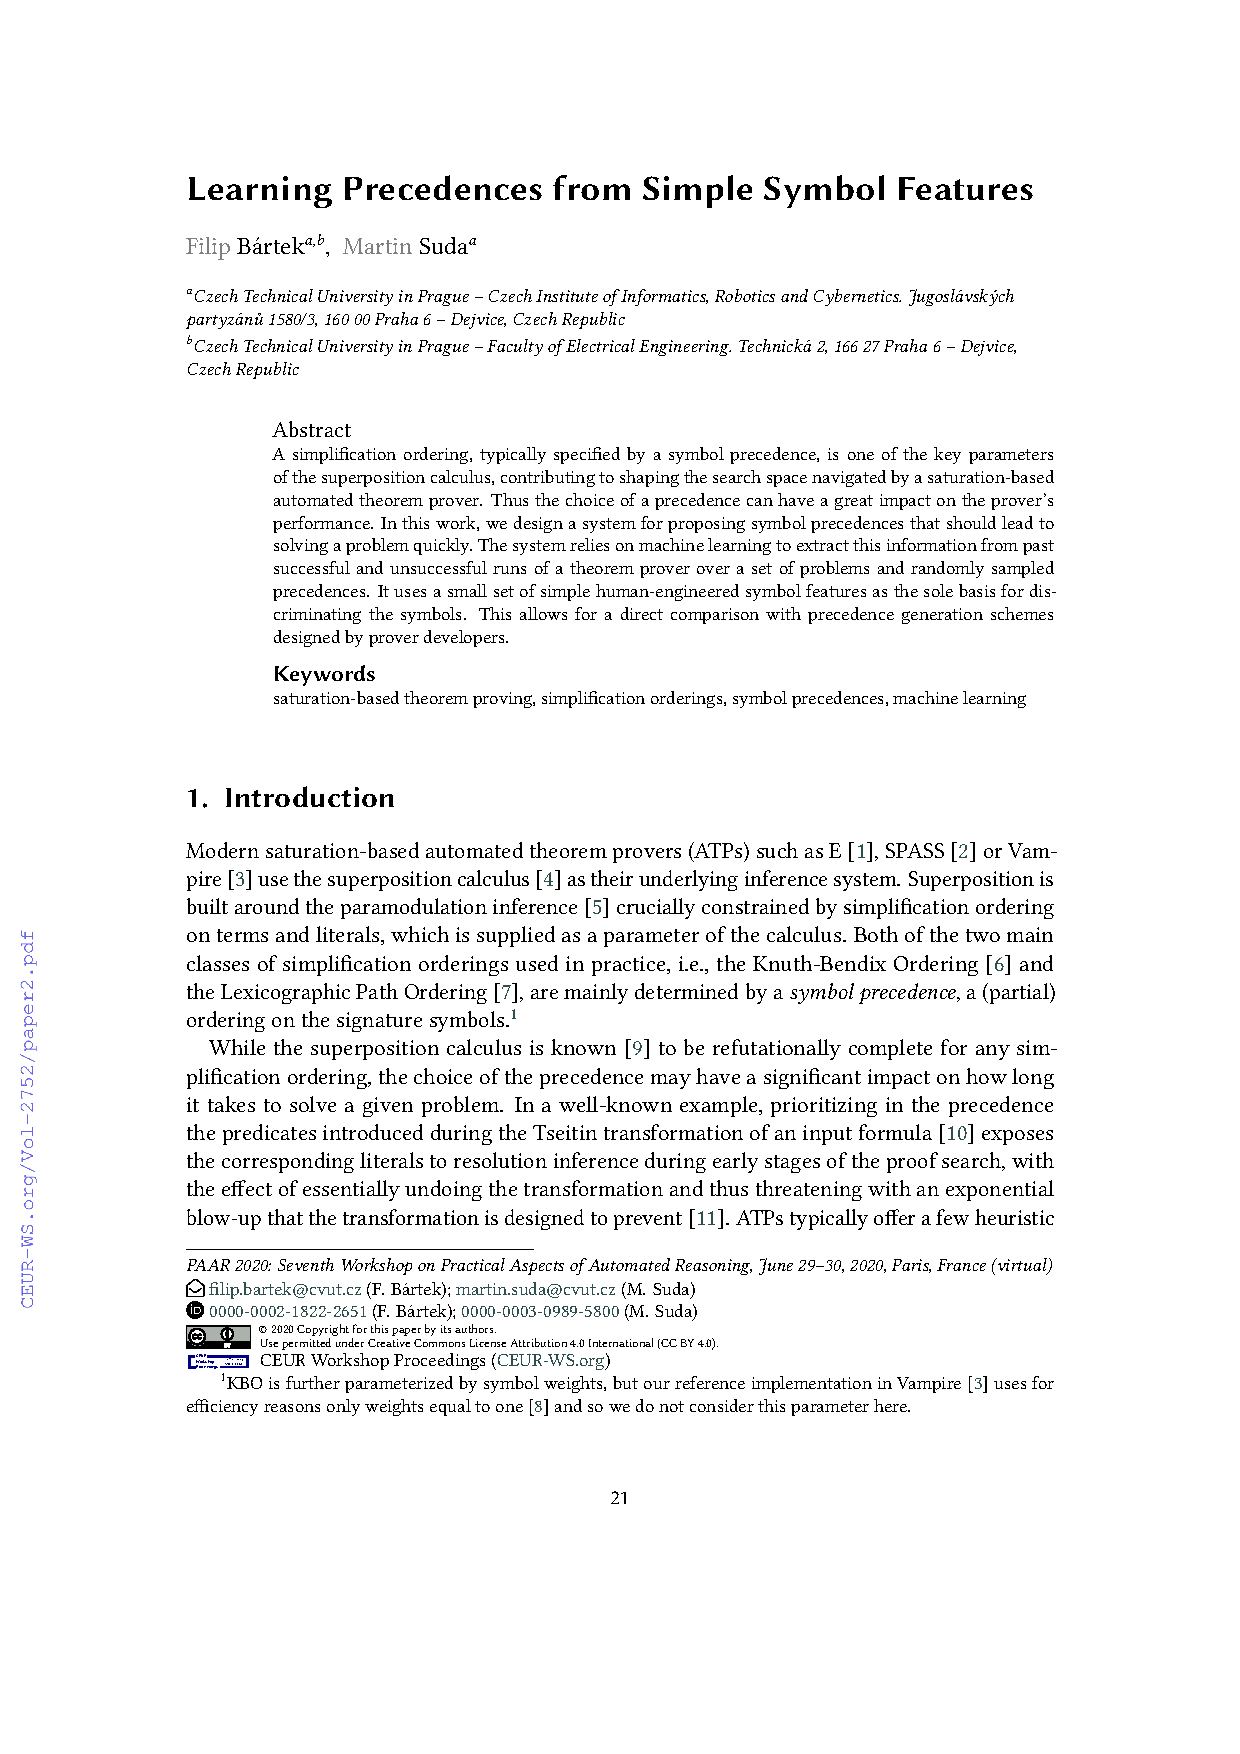
\includepdf[pages=-]{papers/2020-paar.pdf}
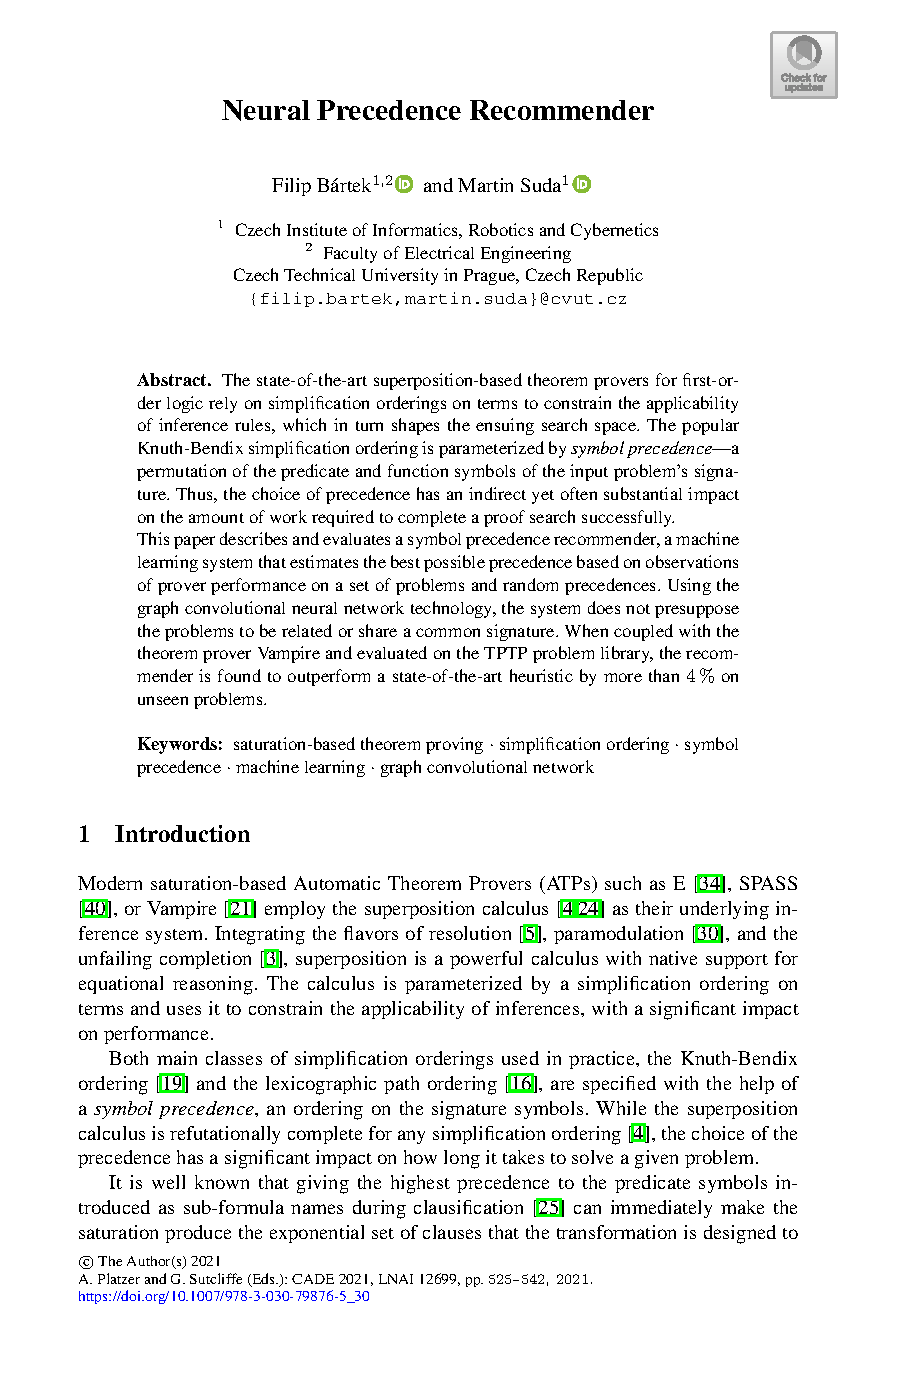
\includepdf[pages=-]{papers/2021-cade.pdf}

\end{document}
